\documentclass[a4paper,14pt]{extarticle}

\usepackage[a4paper,top=20mm,bottom=20mm,left=30mm,right=10mm]{geometry}
\usepackage[T1,T2A]{fontenc}
\usepackage[utf8]{inputenc}
\usepackage[russian]{babel}
\usepackage{indentfirst}
\usepackage{titlesec}
\usepackage{graphicx}
\usepackage{nicematrix}

\renewcommand{\baselinestretch}{1.3}
\titleformat{\section}{\normalsize\bfseries}{\thesection}{1em}{}
\titleformat{\subsection}{\normalsize\bfseries}{\thesection}{1em}{}
\setlength{\parindent}{12.5mm}

\begin{document}
	
	\newpage\thispagestyle{empty}
	\begin{center}
		\MakeUppercase{
			Министерство науки и высшего образования Российской Федерации\\
			Федеральное государственное бюджетное образовательное учреждение высшего образования\\
			<<Вятский Государственный Университет>>\\
		}
		Институт математики и информационных систем\\
		Факультет автоматики и вычислительной техники\\
		Кафедра электронных вычислительных машин
	\end{center}
	\vfill
	
	\begin{center}
		Отчет по лабораторной работе №7\\
		по дисциплине\\
		<<Информатика>>\\
		<<Построение комбинационных схем>>\\
		Вариант 10
	\end{center}
	\vfill
	
	\noindent
	\begin{tabular}{ll}
		Выполнил студент гр. ИВТб-1301-05-00 \hspace{5mm} &
		\rule[-1mm]{25mm}{0.10mm}\,/Макаров С.А./\\
		
		Руководитель доцент кафедры ЭВМ & \rule[-1mm]{25mm}{0.10mm}\,/Коржавина А.С./\\
	\end{tabular}
	
	\vfill
	\begin{center}
		Киров 2024
	\end{center}
	
	\newpage
	\section*{Цель}
	Цель лабораторной работы: закрепить на практике знания о минимизации системы булевых функций и получить навыки реализации простейших арифметических устройств.
	
	\section*{Задание}
	\begin{enumerate}
		\item Выполнить минимизацию булевых функций, представить функции различных базисах – основном логическом базисе (И, ИЛИ, НЕ) или в базисе Шеффера (И-НЕ) в соответствии с вариантом, после чего построить схему в системе Logisim и выполнить проверку.
		
		\item Построить четырехразрядный полный сумматор, складывающий 2 двоичных четырехразрядных числа и учитывающий единицу переноса. Построить схему сумматора в Logisim, проверить его работоспособность.
		
		\item Построить четырехразрядный умножитель, перемножающий 2 двоичных четырехразрядных числа. Построить схему умножителя в Logisim, проверить его работоспособность.  Допускается использование следующих логических элементов: И, ИЛИ, НЕ, И-НЕ, ИЛИ-НЕ,  сложение по модулю 2, эквивалентность.
		
		\item Построить 16-разрядный сумматор со схемами ускоренного переноса.  Построить схему сумматора в Logisim, проверить его работоспособность.  Допускается использование следующих логических элементов: И, ИЛИ, НЕ, И-НЕ, ИЛИ-НЕ,  сложение по модулю 2, эквивалентность.
	\end{enumerate}
	
	\newpage
	\section*{Решение}
	\subsection*{Задание 1}
	Таблица истинности для функции 1 представлена на таблице 1.
	
	\noindent Таблица 1 -- Таблица истинности функции 1 \\
	\begin{NiceTabular}{cccc}[hvlines]
		$x_1$ & $x_2$ & $x_3$ & $f$ \\
		0 & 0 & 0 & 0 \\
		0 & 0 & 1 & 0 \\
		0 & 1 & 0 & 0 \\
		0 & 1 & 1 & 1 \\
		1 & 0 & 0 & 1 \\
		1 & 0 & 1 & 0 \\
		1 & 1 & 0 & 0 \\
		1 & 1 & 1 & 1
	\end{NiceTabular}\\
	
	Диаграмма Вейча-Карно для минимизации функции 1 представлена на таблице 2.
	
	\noindent Таблица 2 -- Диаграмма Вейча-Карно функции 1 \\
	\begin{NiceTabular}{cccccc}[hvlines]
		& $x_2$ & 0 & 0 & 1 & 1 \\
		& $x_3$ & 0 & 1 & 1 & 0 \\
		$x_1$ & & & & & \\
		0 & & & & 1 & \\
		1 & & 1 & & 1 &
	\end{NiceTabular} \\
	
	Минимизированная функция: $f=x_1\overline{x}_2\overline{x}_3\lor x_2x_3$. Комбинационная схема представлена на рисунке 1.
	
	\begin{figure}[h]
		\centering
		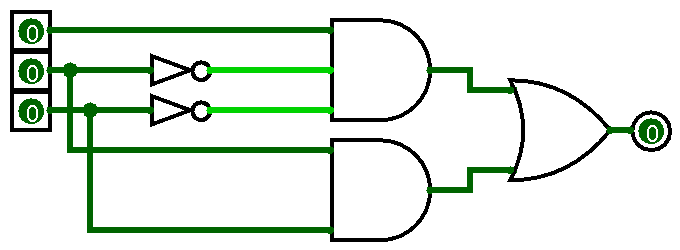
\includegraphics[width=0.5\linewidth]{images/s-1-1}
	\end{figure}
	\begin{center}
		Рисунок 1 – Комбинационная схема функции 1
	\end{center}
	
	\pagebreak
	Таблица истинности для функции 2 представлена на таблице 3.
	
	\noindent Таблица 3 -- Таблица истинности функции 2 \\
	\begin{NiceTabular}{cccc}[hvlines]
		$x_1$ & $x_2$ & $x_3$ & $f$ \\
		0 & 0 & 0 & 0 \\
		0 & 0 & 1 & 0 \\
		0 & 1 & 0 & 1 \\
		0 & 1 & 1 & 1 \\
		1 & 0 & 0 & 1 \\
		1 & 0 & 1 & 1 \\
		1 & 1 & 0 & 0 \\
		1 & 1 & 1 & 0
	\end{NiceTabular}\\
	
	Диаграмма Вейча-Карно для минимизации функции 2 представлена на таблице 4.
	
	\noindent Таблица 4 -- Диаграмма Вейча-Карно функции 2 \\
	\begin{NiceTabular}{cccccc}[hvlines]
		& $x_2$ & 0 & 0 & 1 & 1 \\
		& $x_3$ & 0 & 1 & 1 & 0 \\
		$x_1$ & & & & & \\
		0 & & & & 1 & 1 \\
		1 & & 1 & 1 & &
	\end{NiceTabular}\\
	
	Минимизированная функция в базисе Шеффера: $f=x_1\overline{x}_2\lor\overline{x}_1x_2=\overline{
		\overline{x_1\overline{x_2x_2}}\;
		\overline{\overline{x_1x_1}x_2}
	}$. Комбинационная схема представлена на рисунке 2.
	
	\begin{figure}[h]
		\centering
		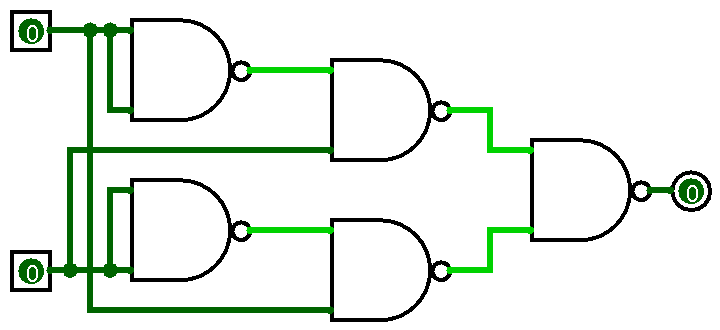
\includegraphics[width=0.5\linewidth]{images/s-1-2}
	\end{figure}
	\begin{center}
		Рисунок 2 – Комбинационная схема функции 2
	\end{center}
	
	\pagebreak
	Таблица истинности для функции 3 представлена на таблице 5.
	
	\noindent Таблица 5 -- Таблица истинности функции 3 \\
	\begin{NiceTabular}{ccccc}[hvlines]
		$x_1$ & $x_2$ & $x_3$ & $x_4$ & $f$ \\
		0 & 0 & 0 & 0 & 1 \\
		0 & 0 & 0 & 1 & 1 \\
		0 & 0 & 1 & 0 & 0 \\
		0 & 0 & 1 & 1 & 0 \\
		0 & 1 & 0 & 0 & 1 \\
		0 & 1 & 0 & 1 & 0 \\
		0 & 1 & 1 & 0 & 0 \\
		0 & 1 & 1 & 1 & 0 \\
		1 & 0 & 0 & 0 & 1 \\
		1 & 0 & 0 & 1 & 0 \\
		1 & 0 & 1 & 0 & 1 \\
		1 & 0 & 1 & 1 & 0 \\
		1 & 1 & 0 & 0 & 1 \\
		1 & 1 & 0 & 1 & 1 \\
		1 & 1 & 1 & 0 & 0 \\
		1 & 1 & 1 & 1 & 1
	\end{NiceTabular}\\
	
	Диаграмма Вейча-Карно для минимизации функции 3 представлена на таблице 6.
	
	\noindent Таблица 6 -- Диаграмма Вейча-Карно функции 3 \\
	\begin{NiceTabular}{ccccccc}[hvlines]
		& & $x_3$ & 0 & 0 & 1 & 1 \\
		& & $x_4$ & 0 & 1 & 1 & 0 \\
		$x_1$ & $x_2$ & & & & & \\
		0 & 0 & & 1 & 1 & & \\
		0 & 1 & & 1 & & & \\
		1 & 1 & & 1 & 1 & 1 & \\
		1 & 0 & & 1 & & & 1 \\
	\end{NiceTabular} \\
	
	Минимизированная функция: $f=x_1x_2x_4\lor x_1\overline{x}_2\overline{x}_4\lor \overline{x}_1\overline{x}_2\overline{x}_3\lor \overline{x}_3\overline{x}_4$. Комбинационная схема представлена на рисунке 3.
	
	\pagebreak
	\begin{figure}[h]
		\centering
		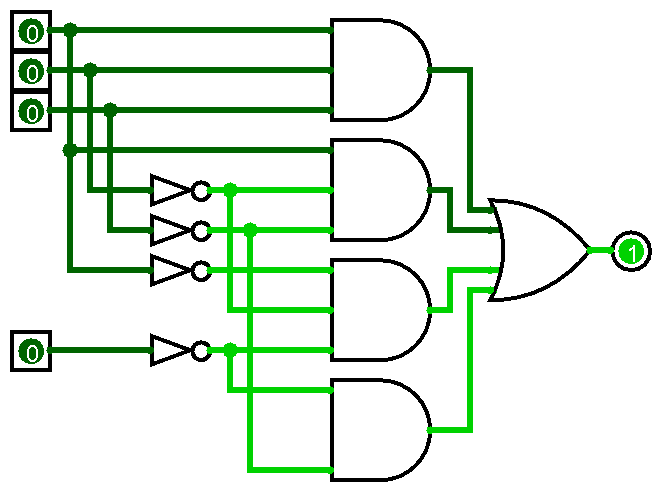
\includegraphics[width=0.5\linewidth]{images/s-1-3}
	\end{figure}
	\begin{center}
		Рисунок 3 – Комбинационная схема функции 3
	\end{center}
	
	Таблица истинности для функции 4 представлена на таблице 7.
	
	\noindent Таблица 7 -- Таблица истинности функции 4 \\
	\begin{NiceTabular}{ccccc}[hvlines]
		$x_1$ & $x_2$ & $x_3$ & $x_4$ & $f$ \\
		0 & 0 & 0 & 0 & 1 \\
		0 & 0 & 0 & 1 & 0 \\
		0 & 0 & 1 & 0 & 0 \\
		0 & 0 & 1 & 1 & 1 \\
		0 & 1 & 0 & 0 & 0 \\
		0 & 1 & 0 & 1 & 1 \\
		0 & 1 & 1 & 0 & 0 \\
		0 & 1 & 1 & 1 & 0 \\
		1 & 0 & 0 & 0 & 1 \\
		1 & 0 & 0 & 1 & 0 \\
		1 & 0 & 1 & 0 & 0 \\
		1 & 0 & 1 & 1 & 1 \\
		1 & 1 & 0 & 0 & 1 \\
		1 & 1 & 0 & 1 & 0 \\
		1 & 1 & 1 & 0 & 1 \\
		1 & 1 & 1 & 1 & 1
	\end{NiceTabular}\\
	
	\pagebreak
	Диаграмма Вейча-Карно для минимизации функции 4 представлена на таблице 8.
	
	\noindent Таблица 8 -- Диаграмма Вейча-Карно функции 4 \\
	\begin{NiceTabular}{ccccccc}[hvlines]
		& & $x_3$ & 0 & 0 & 1 & 1 \\
		& & $x_4$ & 0 & 1 & 1 & 0 \\
		$x_1$ & $x_2$ & & & & & \\
		0 & 0 & & 1 & & 1 & \\
		0 & 1 & & & 1 & & \\
		1 & 1 & & 1 & & 1 & 1 \\
		1 & 0 & & 1 & & 1 & \\
	\end{NiceTabular} \\
	
	Минимизированная функция в базисе Шеффера:\\
	$f=\overline{
		\overline{\overline{x_1x_1}x_2\;\overline{x_3x_3}x_4}\;
		\overline{\overline{x_2x_2}\;\overline{x_3x_3}\;\overline{x_4x_4}}\;
		\overline{x_1\overline{x_3x_3}\;\overline{x_4x_4}}\;
		\overline{x_1x_2x_3}\;
		\overline{\overline{x_2x_2}x_3x_4}\;
		\overline{x_1x_3x_4}
	}$. Комбинационная схема представлена на рисунке 2.
	
	\begin{figure}[h]
		\centering
		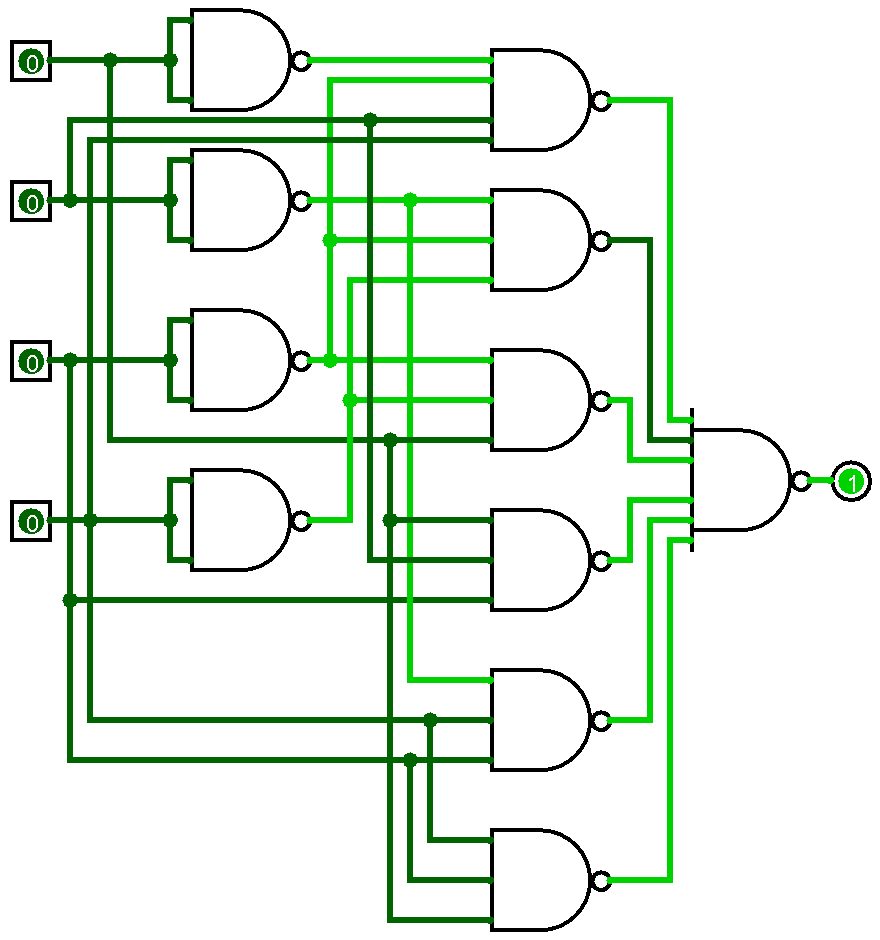
\includegraphics[width=0.5\linewidth]{images/s-1-4}
	\end{figure}
	\begin{center}
		Рисунок 4 – Комбинационная схема функции 4
	\end{center}
	
	\newpage
	\subsection*{Задание 2}
	Комбинационная схема четырехразрядного сумматора состоит из одноразрядных сумматоров, представленные на рисунке 5. Схема четырехразрядного сумматора представлена на рисунке 6.
	
	\begin{figure}[h]
		\centering
		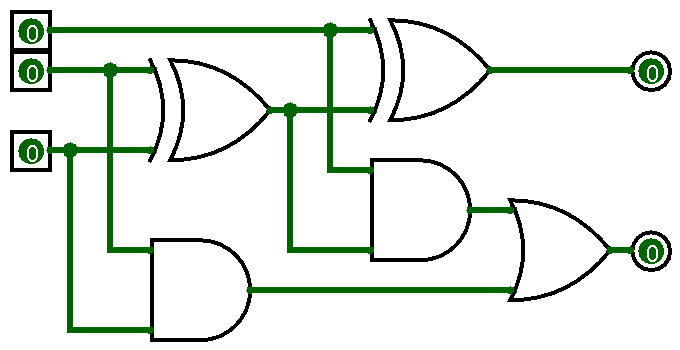
\includegraphics[width=0.5\linewidth]{images/s-2-1}
	\end{figure}
	\begin{center}
		Рисунок 5 – Одноразрядный сумматор
	\end{center}
	
	\begin{figure}[h]
		\centering
		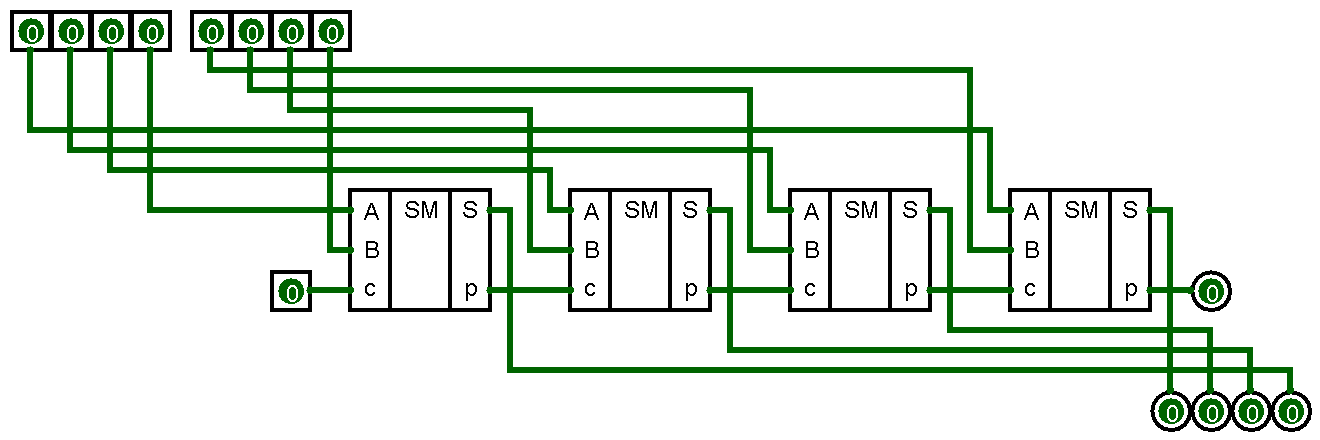
\includegraphics[width=1\linewidth]{images/s-2-2}
	\end{figure}
	\begin{center}
		Рисунок 6 – Четырехразрядный сумматор
	\end{center}
	
	\pagebreak
	\subsection*{Задание 3}
	Комбинационная схема четырехразрядного умножителя представлена на рисунке 7.
	\begin{figure}[h]
		\centering
		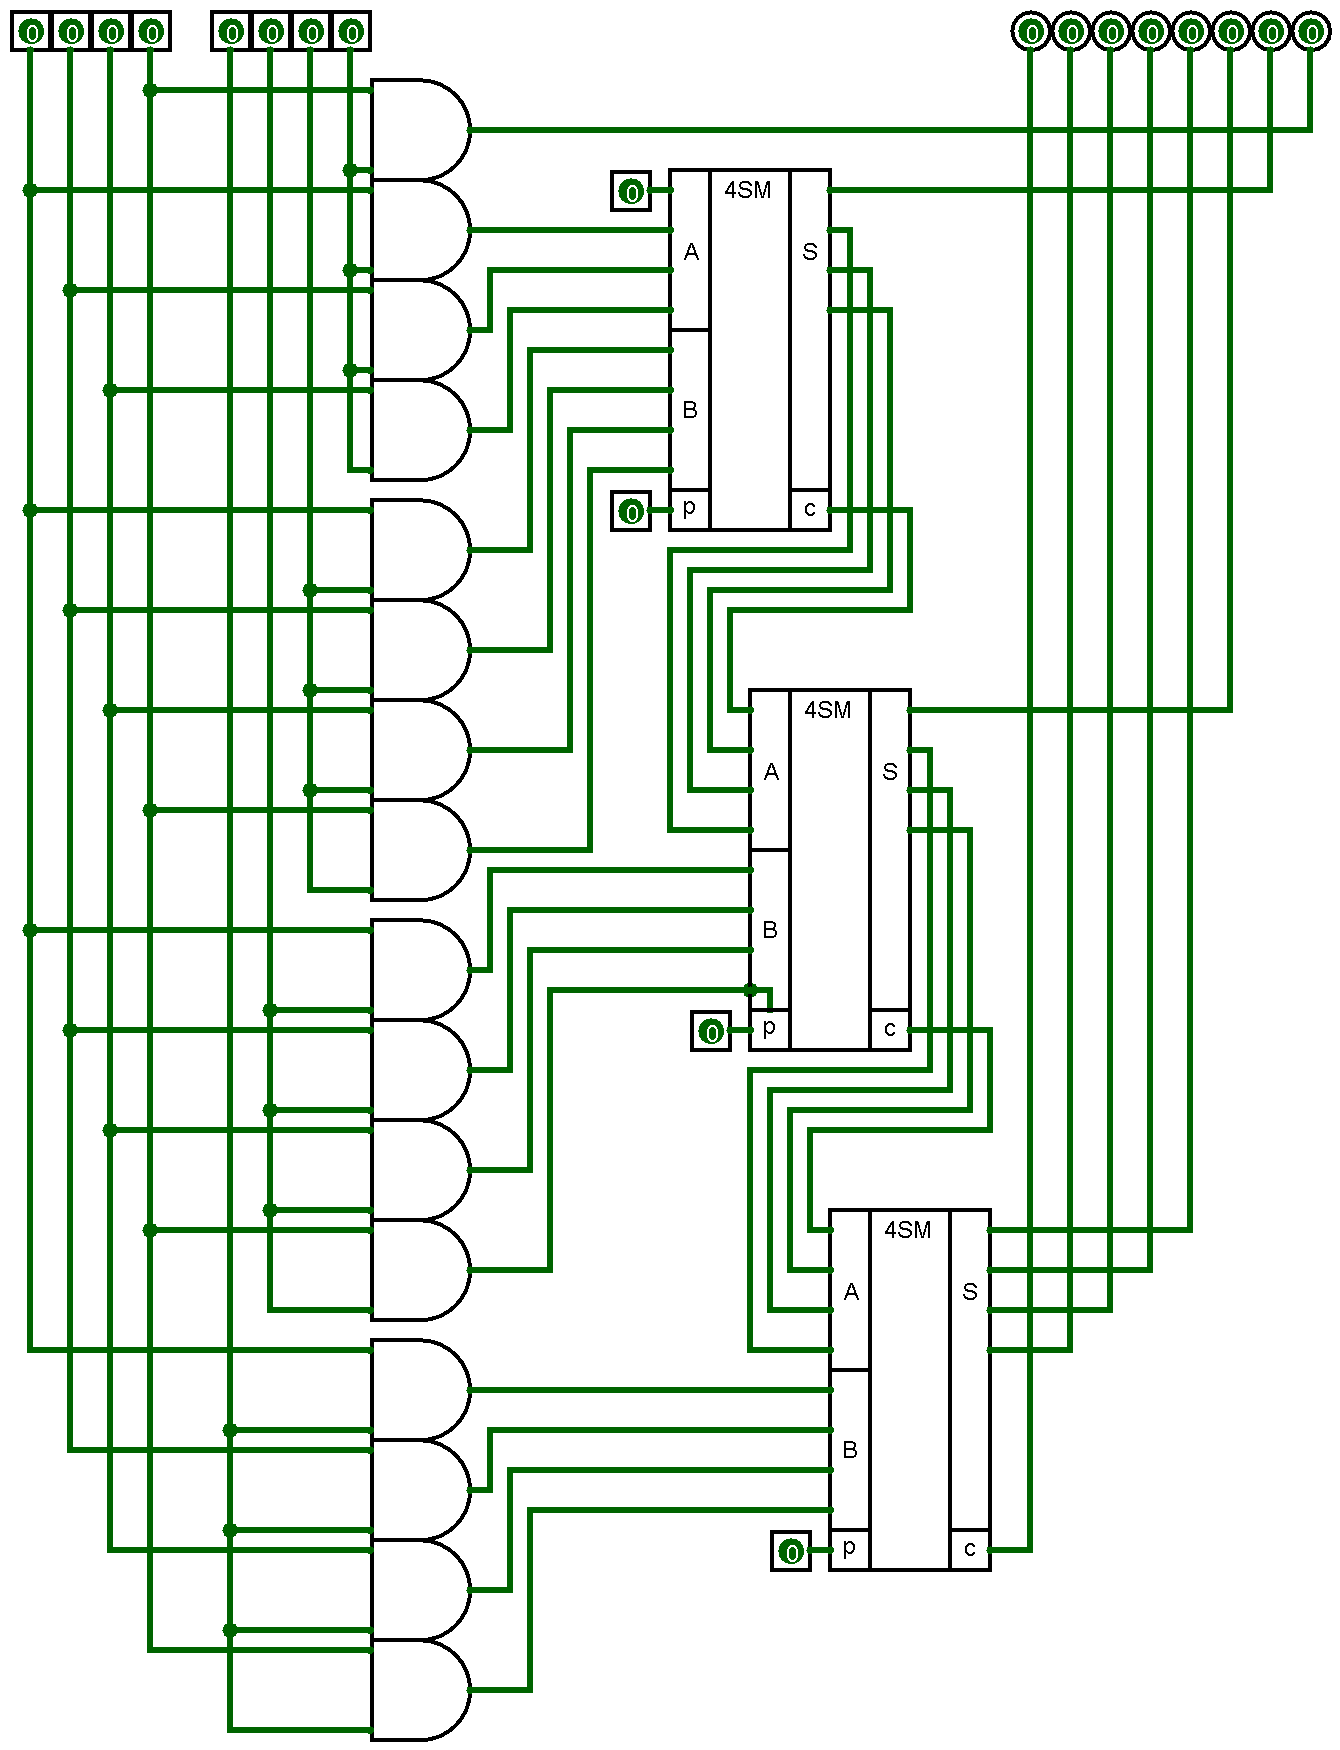
\includegraphics[width=0.9\linewidth]{images/s-3}
	\end{figure}
	\begin{center}
		Рисунок 7 – Четырехразрядный умножитель
	\end{center}
	
	\pagebreak
	\subsection*{Задание 4}
	Комбинационная схема шестнадцати разрядного сумматора с ускоренным переносом представлена на рисунке 8.
	
	\section*{Вывод}
	
\end{document}